\documentclass[11pt]{article}
\usepackage[utf8]{inputenc}
\usepackage{graphicx}
\usepackage{titling}
\usepackage{index}
\usepackage{fancyhdr}
\usepackage{enumitem}
\usepackage{microtype}
\usepackage{blindtext}
\usepackage{amsmath}
\usepackage{wrapfig}
\usepackage{indentfirst}
\usepackage{listings}
\usepackage[labelformat=empty]{caption}
\usepackage{subcaption}
\usepackage[a4paper, total={16cm, 22cm}]{geometry}

\pretitle{
\begin{center}
\vspace{1cm}


\includegraphics[scale=0.2]{FEUP_LOGO.png}

\vspace{2cm}

\LARGE \textbf{SQU}

\vspace{1cm}

}
\posttitle{\end{center}}

\title{
\large{\textbf{Programação em Lógica\\ Relatório Intercalar \\}
Grupo: SQU\_1 \\ \vspace{1cm}\\}}
\author{
  Nuno Miguel Fernandes Marques\\
  \texttt{up201708997@fe.up.pt}
  \and
  Margarida Ribeiro Cosme\\
  \texttt{up201709304@fe.up.pt}
  \\ \vspace{1cm}\\
  }
\date{\today}

\begin{document}
\maketitle
\thispagestyle{empty}

\newpage
\thispagestyle{fancy}
\fancyhf{}
\fancyhead[R]{PLOG - SQU}
\fancyfoot[R]{\thepage}
\renewcommand*{\footrulewidth}{1pt}

\section*{SQU: História e Regras}

\setlength{\parindent}{2ex} 
O SQU é um jogo de tabuleiro para dois jogadores, cada um marcado por uma cor diferente. O material necessário para o jogo são, 50 discos pretos, 50 discos vermelhos, 4 pirâmides pretas, 4 pirâmides vermelhas e um tabuleiro ortogonal 10x10, com um tabuleiro interno de 8x8 em xadrez para facilitar a leitura conforme na figura 1.

\begin{figure}[h]
 \begin{center}
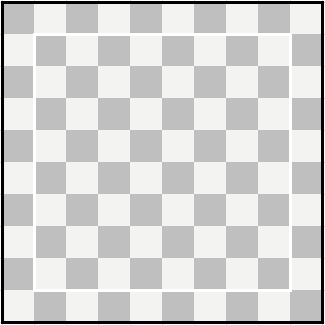
\includegraphics[scale=0.44]{fig1.png}
\caption*{Figura 1: tabuleiro do jogo vazio}
\end{center}
\end{figure}

A cada jogador é atribuída uma cor (vermelho ou preto). Antes de iniciar o jogo, é necessário decidir o tamanho do tabuleiro (8x8 ou 10x10), este começa vazio. Começa o jogador vermelho colocando um disco numa célula vazia do tabuleiro. De seguida joga o jogador preto, os jogadores alternam, colocando dois discos da sua respetiva cor em células vazias.\\

Um “SQU” é um arranjo de quatro discos da mesma cor nos cantos de um quadrado como os lados paralelos aos lados do tabuleiro. O objetivo do jogo é criar o maior “SQU” do tabuleiro. Se, no final da vez de um jogador este formar um “SQU” maior do que qualquer “SQU” existente no tabuleiro, coloca uma pirâmide de sua cor em cada um dos 4 cantos, cobrindo os respetivos discos. Isto é, as pirâmides são usadas para rastrear o maior “SQU” de cada cor. Os discos cobertos por pirâmides ainda podem ser usados para futuros “SQUs”.\\

O jogo termina quando um dos jogadores renunciar, ou quando deixar de haver células livres no tabuleiro. Quando isto acontecer, o jogador com o maior “SQU” ganha (Figura 2). É possível empatar neste jogo (Figura 3). Para a representação do jogo pintamos as células ocupadas por pirâmides completamente.


\begin{figure}[h]
\begin{center}
\begin{subfigure}[b]{0.3\textwidth}
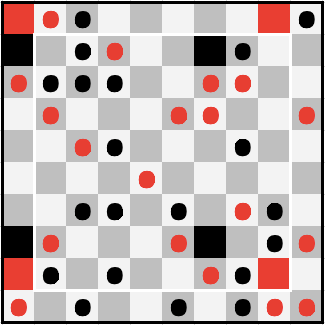
\includegraphics[width=0.9\linewidth, height=3.5cm]{fig2.png}
\caption*{Figura 2: exemplo de jogo vencido pelo jogador vermelho}
\end{subfigure}
\begin{subfigure}[b]{0.3\textwidth}
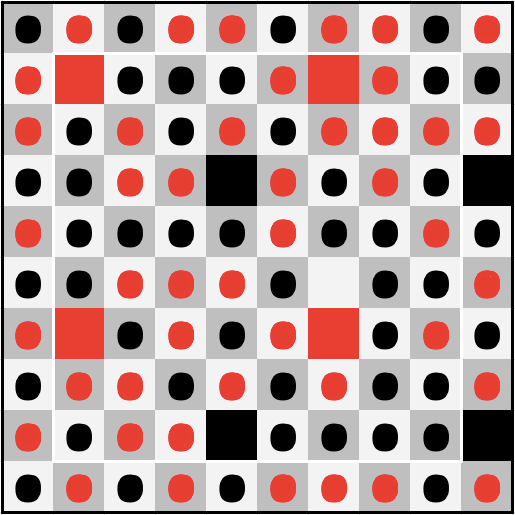
\includegraphics[width=0.9\linewidth, height=3.5cm]{fig3.png}
\caption*{Figura 3: exemplo de jogo empatado}
\end{subfigure}
\begin{subfigure}[b]{0.3\textwidth}
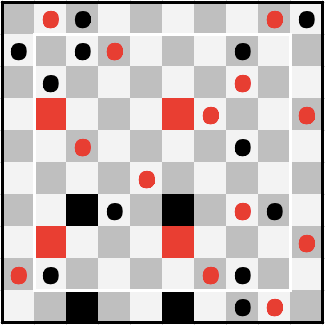
\includegraphics[width=0.9\linewidth, height=3.5cm]{fig4.png}
\caption*{Figura 4: exemplo de uma situação intermédia do jogo}
\end{subfigure}
\end{center}
\end{figure}


\newpage
\thispagestyle{fancy}
\fancyhf{}
\fancyhead[R]{PLOG - SQU}
\fancyfoot[R]{\thepage}
\renewcommand*{\footrulewidth}{1pt}


\section*{Representação Interna do Estado do Jogo}
\begin{center}
Peças:\\
\begin{tabular}{|c|c|}
    \hline
    red  & disco vermelho \\
    \hline
    redp & pirâmide vermelha \\
    \hline
    black & disco preto \\
    \hline
    blackp & pirâmide preta \\
    \hline
\end{tabular} \\
\vspace{1cm}
Exemplos de Representação

\begin{figure}[h]
\begin{center}
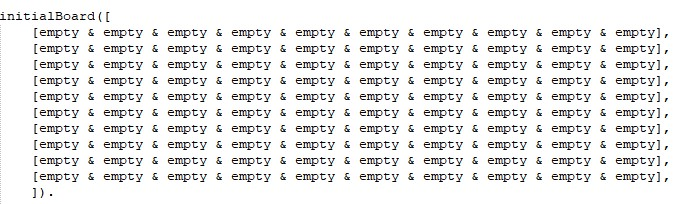
\includegraphics[scale=0.7]{fig5.jpg}
\caption*{Figura 5: Situação Inicial}
\end{center}
\end{figure}

\begin{figure}[h]
\begin{center}
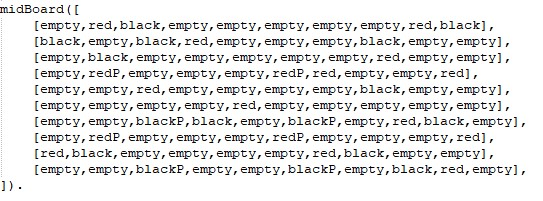
\includegraphics[scale=0.7]{fig6.jpg}
\caption*{Figura 6: Situação Intermédia}
\end{center}
\end{figure}

\begin{figure}[h]
 \begin{center}
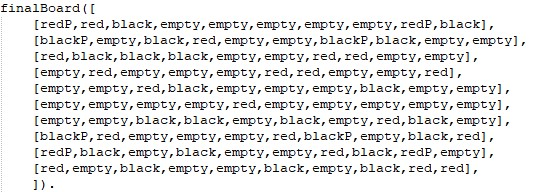
\includegraphics[scale=0.7]{fig7.jpg}
\caption*{Figura 7: Situação Final}
\end{center}
\end{figure}
\end{center}

\newpage
\thispagestyle{fancy}
\fancyhf{}
\fancyhead[R]{PLOG - SQU}
\fancyfoot[R]{\thepage}
\renewcommand*{\footrulewidth}{1pt}

\section*{Visualização do estado de jogo}
O tabuleiro logicamente é uma lista de listas, visualmente o predicado 'display\_game' percorre a lista e imprime um simbolo ,que representa o tipo de peça, para cada elemento da lista. O símbolo a ser usado na visualização e dado chamando 'symbol'. Entre cada linha e coluna são imprimidos separadores e marcadores da linha e coluna.

\begin{figure}[h]
 \begin{center}
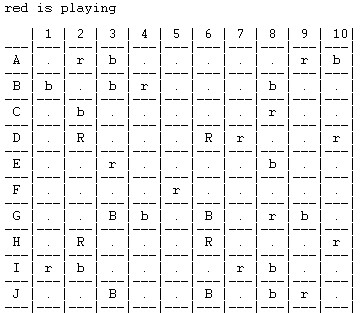
\includegraphics[scale=0.7]{fig8.jpg}
\caption*{Figura 8: Visualização de um jogo em progresso}
\end{center}
\end{figure}


\begin{figure}[h]
 \begin{center}
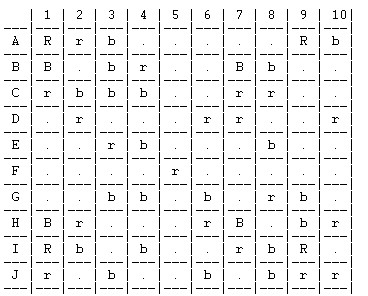
\includegraphics[scale=0.7]{fig9.jpg}
\caption*{Figura 9: Visualização de um jogo acabado}
\end{center}
\end{figure}

\section*{Fontes}
\setlength{\parindent}{} 
•https://nestorgames.com/#squ\_detail \\
•https://boardgamegeek.com/image/5237377/squ

\end{document}

